\section{Machine Intelligence}\label{section:machine-intelligence}
The information of this section is primarily based on the work of \citet{misc:artificial-intelligence}.
Machine intelligence or artificial intelligence is \textit{the field that studies the synthesis and analysis of computational agents that act intelligently} \citep{misc:artificial-intelligence}.
\begin{comment}
An agent observes the environment and acts based on the observations.
For the agent to be considered intelligent, various factors are considered, which will be briefly described hereafter.

A factor to consider is if the agent's actions are appropriate for its environment and its goals. 
An example could be a robot that has to move from point $A$ to point $B$ and there is a straight line to get there. 
If the agent then moves further away from point $B$ instead of reaching it, the agent does not act appropriately.

Another factor which is considered, is if the agent is flexible in changing environments and changing goals. 
An example could be a robot that has to move from point $A$ to point $B$, if an obstacle is blocking the otherwise appropriate path, the agent has to act according to this, thus resulting in another path chosen for the robot to move to point $B$.

In addition to previous factors the agent should learn from experience. 
A case could be a dog that learns to sit when the owner says \textit{sit}. 
Another case could be the agent mentioned above, where if the obstacle has been blocking the shortest path from point $A$ to point $B$ multiple times, the agent will learn from this and therefore avoid that path.

Lastly, the agent has to make appropriate choices given its perceptual and computational limitations.
An example could be an agent that has to answer in a given time frame, and thus will give an answer that may not be the optimal answer, but is a good answer given its computational limitations, since memory is finite and the agent might not be able to observe the state of the world directly.

\begin{figure}[h]
    \centering
    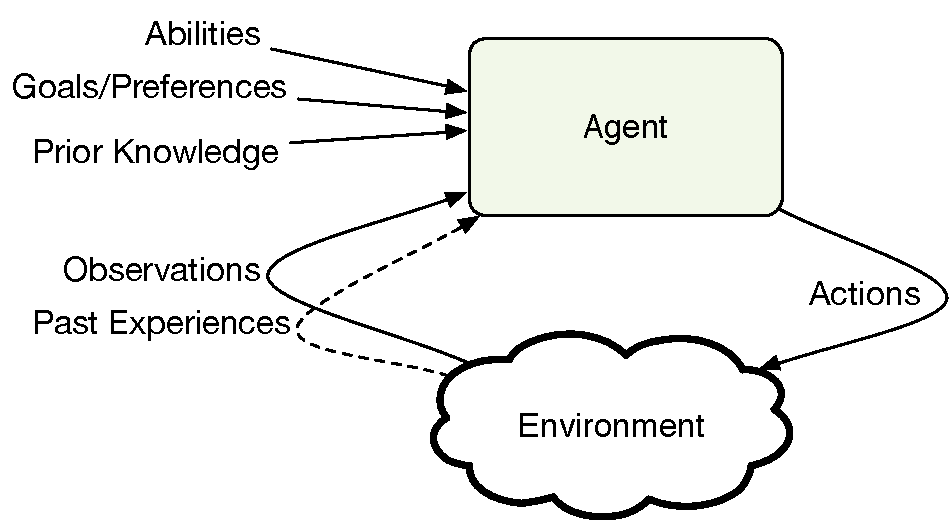
\includegraphics[scale=0.6]{media/agent}
    \caption{An agent and how it interacts with the environment\citep{misc:artificial-intelligence}}
    \label{figure:agent}
\end{figure}

In \figref{figure:agent} the input and output of an agent is shown. 
The agent depends on the following, as written in \citep{misc:artificial-intelligence},

\begin{itemize}
    \item \textbf{prior knowledge} about the agent and the environment;
    \item \textbf{history} of interaction with the environment, which is composed of
    \begin{itemize}
        \item \textbf{observations} of the current environment and
        \item \textbf{past experiences} of previous actions and observations, or other data, from which it can learn;
    \end{itemize}
    \item \textbf{goals} that it must try to achieve or preferences over states of the world; and
    \item \textbf{abilities}, which are the primitive actions it is capable of carrying out.
\end{itemize}

To test whether an agent is truly intelligent or not, the Turing test can be used.
The principal of the Turing test is to determine whether an interrogator is able to identify and distinguish between a human and an agent \citep{misc:machine-intelligence-course}. 
\end{comment}